\section{Diagramme de séquence}

Nous représentons le scénario de la déviation d'une route vers un trou noir en utilisant le diagramme de séquence.
\newline
L'utilisateur de l'application web dans cet exemple est l'administrateur réseaux. On suppose que l'administrateur réseaux veut dévier une route par son adresse IP source. 
\newline
Lorsque l'opération est terminé, donc l'application web confirme que c'est fait, la route est ensuite serait stockée dans la base de données afin que le client puisse aller consulter les routes qui ne sont pas accessibles.
\\
\\

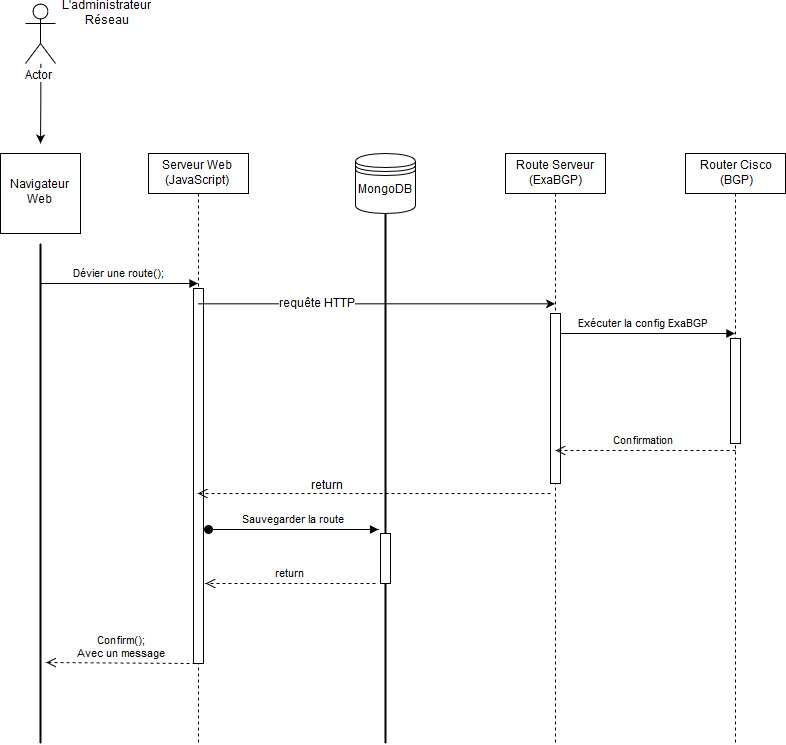
\includegraphics[scale = 0.5]{img/seqDiagramme}
